\documentclass{article}

% if you need to pass options to natbib, use, e.g.:
%     \PassOptionsToPackage{numbers, compress}{natbib}
% before loading neurips_2021

% ready for submission
\usepackage{neurips_2021}

% to compile a preprint version, e.g., for submission to arXiv, add add the
% [preprint] option:
%     \usepackage[preprint]{neurips_2021}

% to compile a camera-ready version, add the [final] option, e.g.:
%     \usepackage[final]{neurips_2021}

% to avoid loading the natbib package, add option nonatbib:
%    \usepackage[nonatbib]{neurips_2021}

\usepackage[utf8]{inputenc} % allow utf-8 input
\usepackage[T1]{fontenc}    % use 8-bit T1 fonts
\usepackage{hyperref}       % hyperlinks
\usepackage{url}            % simple URL typesetting
\usepackage{booktabs}       % professional-quality tables
\usepackage{amsfonts}       % blackboard math symbols
\usepackage{nicefrac}       % compact symbols for 1/2, etc.
\usepackage{microtype}      % microtypography
\usepackage{xcolor}         % colors



\usepackage{amsmath, amsfonts, amsthm}
\usepackage{enumerate}
\usepackage{graphicx}
\usepackage{subcaption}

\theoremstyle{definition}
\newtheorem{definition}{Definition}
\newtheorem{theorem}{Theorem}
\newtheorem{corollary}{Corollary}
\newtheorem{assumption}{Assumption}
\newtheorem*{remark}{Remark}

\newcommand{\ah}[1]{\textcolor{blue}{AH: \textit{#1}}}
\newcommand{\fb}[1]{\textcolor{red}{FB: \textit{#1}}}

\newcommand{\agentset}{\mathcal{N}}
\newcommand{\edgeset}{\mathcal{E}}
\newcommand{\weightset}{W}

\newcommand{\actionset}[1]{S^{#1}}
\newcommand{\utility}[1]{u^{#1}}

\newcommand{\wmunu}{w^{\mu \nu}}
\newcommand{\xmu}{x^{\mu}}
\newcommand{\xnu}{x^{\nu}}
\newcommand{\refmu}{\sigma^{\mu}}
\newcommand{\avgref}[1]{\alpha_\sigma^{#1}}
\newcommand{\NE}[1]{\bar{x}^{#1}}
\newcommand{\weightedsum}{ \sum_{\nu \in N^\mu} \wmunu \xnu}
\newcommand{\xnotmu}{x^{-\mu}}
\newcommand{\xmuaction}[1]{x^{\mu}_{#1}}

\newcommand{\pure}[2]{e^{#1}_{#2}}


\title{Equilibria and Convergence of Fictitious Play on Network Aggregative Games}

% The \author macro works with any number of authors. There are two commands
% used to separate the names and addresses of multiple authors: \And and \AND.
%
% Using \And between authors leaves it to LaTeX to determine where to break the
% lines. Using \AND forces a line break at that point. So, if LaTeX puts 3 of 4
% authors names on the first line, and the last on the second line, try using
% \AND instead of \And before the third author name.

\author{%
 Aamal Hussain  \\
  Department of Computing\\
  Imperial College London\\
  South Kensington, London \\
  \texttt{aamal.hussain15@imperial.ac.uk} \\
  % examples of more authors
  \And
  Francesco Belardinelli
  % Coauthor \\
  % Affiliation \\
  % Address \\
  % \texttt{email} \\
  % \AND
  % Coauthor \\
  % Affiliation \\
  % Address \\
  % \texttt{email} \\
  % \And
  % Coauthor \\
  % Affiliation \\
  % Address \\
  % \texttt{email} \\
  % \And
  % Coauthor \\
  % Affiliation \\
  % Address \\
  % \texttt{email} \\
}

\begin{document}

\maketitle

\begin{abstract}
  Understanding the long term behaviour of learning algorithms is an important object of study if we are to design systems which can be considered safe. However, as the number of players in a game increase, it is known that the dynamics of learning becomes increasingly chaotic. As such, the most rigorous results of learning dynamics are limited to two player games.

  In this study, we contribute towards the study of learning with multiple agents. We do this through the introduction of learning on network aggregative games, in which each player's reward is dependent on its own strategy and a convex combination of its neighbours. In particular, we present a continuous time analysis of the Fictitious Play learning dynamic on such a game. We reach a number of conclusions. In particular, we show that Fictitious Play reaches a fixed point when the game is zero-sum and provide conditions under which this fixed point corresponds to a Nash Equilibrium. In addition, we show that agents learning through Fictitious Play achieve no-regret, regardless of the choice of game. Finally, we present experimental evidence of a family of games for which Fictitious Play reaches a limit cycle and evidence that the introduction of noise has the potential to break this cyclic behaviour and allow agents to reach the Nash Equilibrium.
\end{abstract}

\section{Introduction}

Multi-Agent Learning \cite{Schwartz} requires a number of agents to adapt in an environment where
each agent must adapt in response to the behaviour of the other agents. This leads to a
fundamentally non-stationary problem, which presents a challenge to designing effective learning
policies. Even when there are a small number of agents in the game, learning has been shown to lead
to non-stationary, and even chaotic behaviour \cite{SatoChaos}, and this problem becomes even more
pronounced as the number of agents increase \cite{Sanders}. In this light, it would seem that, when there is a large population of agents, it is almost impossible to understand the long term behaviour of multi-agent learning \cite{PiliourasChaoticMaps}. This, of course, poses a problem for AI safety, for which it is desirable that learning systems are designed so that their ultimate behaviour is guaranteed to satisfy some predetermined goals.

To deal with this problem, one must attempt to reduce the many player game to something which is
tractable. A number of reductions have been proposed, most notably \emph{Mean Field} Games
and \emph{Aggregative} Games. The former makes the assumption of an infinite
number of agents, so that the population can be represented through a distribution over players'
states \cite{CainesPaper} . Every agent then updates their action profiles depending on this
distribution. In the latter each agent considers a real valued function which is a convex
combination of the states of the other agents. Both formulation allows for a many player game to be reduced to a set of two-player games.

Both formulations have been the object of rigorous study and it has been shown that agents reach an equilibrium when learning on such games (c.f. \cite{MFGLearningPapers} for Mean Field Games and
\cite{Aggregative Papers} for Aggregative Games). However, both also present a fundamental limitation.
Namely, they both require that agents have access to the action profiles of the entire population.
This could be through communication with all other agents, or through the intervention of a central
coordinator who is able view the entire population. Whilst recent work aims to relax this assumption
through the introduction of noise \cite{MFG-FP} or partial observability \cite{AAMASPaper}, the
requirement that each agent updates their actions based on the entire population is rather strong and not always supported by empirical evidence.

In this study, we investigate a variant of the aggregative game known as the \emph{Network
Aggregative} (NA) Game. This format assumes that there is an underlying communication network
through which agents interact. Then each agent updates their actions according only to those agents
with whom they communicate. This significantly relaxes the communication load on each agent and
lifts the need for a central coordinator. Recent work on the NA game has shown that it is possible
for agents to reach an equilibrium strategy in an entirely distributed manner \cite{Grammatico,
LeaderFollower, MyopicAgents}. We contribute in this direction by analysing the long term behaviour of learning on an NA game. In particular, we analyse the Fictitious Play Learning
Algorithm \cite{Brown, Harris}, in which agents are assumed to be myopic, in that they react solely
to the previous behaviour of the others.


\subsection{Contributions}

  The main contribution of this work is to introduce learning on the Network Aggregative Game
  through the action of Fictitious Play (FP).

  We first show that, in aggregative games played with FP, a Nash Equilibrium exists and that FP admits
  solutions in this setting. In particular, we study zero-sum games and show that
  FP converges to a fixed point, which for a network without any
  self-loops corresponds to a Nash Equilibrium. In addition, we find that, for games
  which are not zero-sum, agents following FP are able to
  achieve no regret.

  Finally, we explore FP through numerical simulations to consider the
  question of whether it always converges. We answer this in the negative by finding a family of
  games in which action profiles cycle around the Nash Equilibrium. Finally, our experiments
  document how noise affects the convergence of FP. Our experiments suggest that, under
  the presence of noise, the algorithm still reaches a fixed point, but perhaps not the Nash
  Equilibrium. This presents an interesting avenue for future research.

\subsection{Related Work}

\paragraph{Network Aggregative Games}

The NA game is a recent introduction \cite{Parise2015} which presents a variant of aggregative games
by adding an underlying structure to the population. Since its introduction, distributed algorithms
have been built with the aim of finding NE. In particular, \cite{Parise2015, Parise2020} consider
the case in which payoffs are given by Lipschitz functions with unique minimisers and apply standard
topological fixed point towards designing algorithms which will converge to the NE. We note that the
\emph{Mann Iteration}, one of the algorithms applied in \cite{Parise2020} shares a remarkably
similar form with the discrete variant of FP. To the best of our knowledge, this link has not been
explored in the literature and is an avenue for research which we are currently pursuing. Another
common algorithm for distributed NE seeking is the projected gradient (resp. subgradient) dynamics
which is explored in \cite{Zhang2020} (resp. \cite{Shokri2020, Shokri2021}). In all of these works,
the cost function is assumed to be convex, and therefore have a unique minimiser. In fact this is a
common assumption in works concerning NA Games \cite{Zhu2021, Lei2020}, which we believe is due to
its ubiquity in control settings. We have not yet come across works which consider NA games from the
point of view of payoff matrices, which are more common in multi-agent learning settings.
Furthermore, to the best of our knowledge, this is the first work which introduces the application
of a learning algorithm in the NA setting.

\paragraph{Fictitious Play}

Fictitious Play was introduced by Brown in 1951 \cite{BrownPublished, BrownUnpublished} as a
'natural' way in which to approximate the Nash Equilibrium in zero sum games. It was known at the
time that a discrete variant of the algorithm would converge to the NE in two player zero-sum games
\cite{Robinson}. Since then a number of proofs of convergence were determined in 2 player games
\cite{Miyasawa, Polak, Berger, Monderer and Sela, Monderer and Shapley}, as well as corresponding
convergence rates \cite{Harris, Shapiro}. Many results hold for both the discrete and continuous
variants of FP. Their relation was finally solved by Hofbauer \cite{Hofbauer}, who showed that
attractors of the discrete time process are also attractors for the continuous time variant. As
such, most of the analysis on FP focuses on the continuous time variant \cite{Ostrovski}. It was
later shown in \cite{Shapley} that there is a family of games (now called the \emph{Shapley family})
for which FP does not converge at all but rather shows periodic behaviour. However, the work looking at fictitious play
where there are more than two agents is sparse. \cite{Sela} considers a game in which a multi-player
game is decomposed by requiring that each agent engage in a two person game against each of the
opponent. Their payoff is given by the sum of payoffs in all of these subgames. It was found that,
if this game is zero sum, then FP will converge. Similar results for more than two players were
found for games where all agents share the same payoff in \cite{MondererShapley1994}. In \cite{FPMFG}, the action
of FP was considered in a Mean Field Game, and it was found again that the algorithm converges for
zero sum games. The most general result, and the one most similar to our own, was found by Ewerhart
and Valkanova in 2020 \cite{Ewerhart} in which they showed that fictitious play converges in network
games, where each agent is engaged in a two-player game with each of their neighbours. The rate of
convergence was found to be independent of the network size.  Our work extends the analysis of FP in
multiplayer games by considering its action in NA Games, so that the agents do not play individual
games against each of their neighbours but rather a single game against the aggregate of their
neighbours. In particular we also extend a result for two player games found by Ostrovski and van
Strein \cite{Payoff Performance} which showed that FP achieves no-regret to the multi-player
setting.

\section{Preliminaries}
In this section we introduce the network aggregative game framework, as well as defining FP on such a game.

\subsection{Network Aggregative Games}
\label{sec::NAG}

  The model we consider is that there is a set $\agentset = {1,
           \ldots , N}$ of agents who are connected through an underlying
          interaction graph. This graph is given by the tuple
          $(\agentset, (\edgeset, \weightset))$ in which $\edgeset$ is
          the set of all pairs $(\mu, \nu) \in \agentset \times \agentset$
          connected. Formally,
        
  \begin{definition}[Interaction Graph]
    Given a set $\agentset$ of agents, an {\em interaction graph} $I = (\agentset, (\edgeset,
    \weightset))$ such that
    \begin{itemize}
    \item $\edgeset \subseteq \agentset \times \agentset$.        Then, the set of neighbours of agent
        $\mu$ is denoted as $N^\mu = \{\nu \in \agentset \, : \, (\mu, \nu) \in \edgeset\}$.
      \item $\weightset \in M_N(\mathbb{R})$ is the weighted adjacency matrix whose elements $w^{\mu
        \nu}$ expresses the importance that agent $\mu$ places on agent $\nu$. If $(\mu, \nu) \not
        \in \edgeset$ then $w^{\mu \nu} = 0$;        $\wmunu \in (0, 1]$ otherwise.
    \end{itemize}
  \end{definition}

  With the above definition, we can formalise the network aggregative (NA) game:

  \begin{definition}[Network Aggregative Game]
    A Network Aggregative game is defined as the tuple $\Gamma = (I, (\actionset{\mu},
        \utility{\mu})_{\mu \in \mathcal{N}})$, where $I$ is the interaction graph,
        $\actionset{\mu}$ and $\utility{\mu}$ refer to $\mu$'s set of actions (with cardinality
        $|\actionset{\mu}| = n$) and utility function respectively.
  \end{definition}

  We consider the \emph{state} of agent $\mu$ to be the probability vector $\xmu \in
  \mathbb{R}^n$ where $\xmu_i$ is the probability with which the agent plays action $i$. It
  should be noted that this probability vector is often referred to as $\mu$'s \emph{mixed
  strategy}. With this in mind, we can construct, as their state space, the unit simplex on
  agent $\mu$'s action set. This is given as $\Delta_\mu := \{\xmu \in \mathbb{R}^n \, : \,
  \sum_i \xmuaction{i} = 1\}$. Also associated with each agent is a utility function

  The utility function, for each agent $\mu$, is given as $u^\mu(\xmu, \xnotmu)$ in which we use
  the standard notation $-\mu$ to refer to all agents other than $\mu$. Notice that this requires
  that each agent play the same strategy against all of their neighbours. What is unique about the
  NA game is the structure of the payoffs themselves. In this format, each agent is receives a
  reference $\sigma$ which is a weighted sum of each of their neighbours
  state. Formally
  %
  \begin{equation}
    \sigma^\mu = \sum_{\nu \in N^\mu} \wmunu \xnu.
  \end{equation}

  Then, the agent's must optimise their payoff with respect to this reference vector. Thus,
  instead of having to consider the actions of the entire population, or play individual games
  against each of their neighbours, the agent only has to consider $\sigma^\mu$ as a
  `measurement' of the local aggregate state and optimise with respect to this measurement.
  This allows us to make the reduction $u^\mu(\xmu, \xnotmu) = u^\mu(\xmu, \refmu)$. In
  particular, we consider that the agent is engaged in a matrix game against the
  reference vector so that
  %
  \begin{equation}
    u^\mu(\xmu, \refmu) = \xmu \cdot A^\mu \refmu = \xmu
                \cdot A^\mu \weightedsum.
  \end{equation}

  where $A^\mu$ is the payoff matrix associated to agent $\mu$. Note that this means we can write
  the game $\Gamma$ with the payoff matrices $A^mu$ in place of the utility functions
  $\utility{\mu}$. The NA game allows for the reduction of a multiplayer game into a series of
  two-player games. The agent's goal is to maximise their payoff with respect to the reference
  vector. As such, we define the best response correspondence $BR^\mu$ which maps any $\refmu$
  the set $\arg \max_{y \in \Delta_\mu} {u^\mu(y, \refmu)}$. 

  Finally, a central concept of game theory is that of the Nash Equilibrium, in which no rational
  agent has the incentive to deviate from their current state. This can be formalised by saying
  that all agents are playing the best response to each other.

  This leads naturally to the definition of a Nash Equilibrium in an NA Game as

  \begin{definition}(NE) \label{def::NE}
    The set of vectors $\{ \NE{\mu}\}_{\mu \in \agentset}$ is an NE if, for all $\mu$,  
    \begin{equation*}
    \NE{\mu} \in BR^\mu (\refmu) = \arg \max_{x \in \Delta_\mu} u^\mu(x, w^{\mu \mu} x + \sum_{\nu \in N^\mu \backslash \{\bar{\mu}\}} \wmunu \NE{\nu}).
    \end{equation*} 
  \end{definition}
    
  \begin{remark}
    It can be seen that the concept of the Nash Equilibrium in the NA game is a natural
    extension of the NE in a bimatrix game $(A, B)$. In particular, if we consider an NA game
    with only two players and no self-loops then the above definition yields

    \begin{equation*}
      \NE{1} \in BR^1 (\sigma^1) = \arg \max_{x in \Delta_1} u^1 (x, \NE{2}), 
    \end{equation*}

    and similarly for $\NE{2}$. This is precisely the definition of an NE in a two player game \cite{}.
  \end{remark}

  We will show that the NE exists for an NA game in Section \ref{sec::ExistenceofNE}. 

  Finally we note that an NA game is \emph{zero-sum} if the utilities of each agent sum to zero for any strategy set $\{ \xmu \}_{\mu \in \agentset}$. Formally

  \begin{equation}
    \sum_\mu u^\mu(\xmu, \weightedsum) = 0.
  \end{equation}

\subsection{Continuous Time Fictitious Play}
\label{sec::CTFP}

  Fictitious Play requires that, at the current time, each agent considers the average state
  of their opponent in the past, and respond optimally (i.e. play a best response) to this state. In the case of an NA game, each agent considers their reference vector to be their
  opponent. As such, each agent $\mu$ must update their state according to the time-average of
  $\refmu$. To formalise this we write

  \begin{equation}
    \avgref{\mu} = \frac{1}{t} \int_0^t \refmu(s) \; ds.
  \end{equation}

  Using this, we follow in the footsteps of Ewerhart \cite{} and Harris \cite{} to define
  Fictitious Play in continuous time, but with a slight adaptation for the NA game.
%
  \begin{definition}[Network Aggregative - Continuous Time Fictitious Play (NA-CTFP)]
    An NA-CTFP is defined as a measurable map $m$ with components $m^\mu$ such that for all $\mu$
    and all $t \geq 1$, $m^\mu: [0, \infty) \rightarrow \Delta_\mu$ satisfies $m^\mu(t) \in
    BR^\mu(\alpha_{\sigma}^\mu)$ for almost all $t \geq 1$.
  \end{definition}

  We can think of this definition as saying that the player plays some arbitrary strategy before
  $t = 1$, but beyond this it must play a best response to the time average of its reference
  signal.
  
  \begin{remark}
    As an illustration, consider the NA game with two players, in which $\edgeset = \{(1, 2),
    (2, 1)\}$ and $\weightset$ is a 2x2 matrix with zeros on its leading diagonal and ones on
    the off diagonal. We write the time-average of both agents' state as
  
    \begin{align}
      \alpha^\mu(t; x) = \frac{1}{t} \int_0^T \xmu(t) \, dt & \text{ for $\mu \in \{1, 2\}$}
  %   \alpha^2 = \frac{1}{t} \int_0^T x^2(t) \, dt \\
    \end{align}

    In this manner, the $\alpha^\mu(t; m)$ denotes the time average of the strategies played by
    agent $\mu$ up to time $t$ when the strategies are given by $\xmu(t)$. Note that we often reduce the notation to $\alpha^\mu(t)$. Then, fictitious play requires that the agents update their
    strategy as $x^1(t) \in BR^1(\alpha^2(t))$ and $x^2(t) \in BR^2(\alpha^1(t))$. It can be
    seen, therefore, that the NA-CTFP is a natural extension of CTFP in the classical
    two-player setting \cite{}.
  \end{remark}

\subsection{Assumptions}

  With the above preliminaries in place, we can state the assumptions that we make in this study.

  \begin{assumption}\label{ass::rowstochastic}
    The weighted adjacency matrix $\weightset$ is constant and \emph{row stochastic} meaning
    that the sum elements in each row of $\weightset$ is equal to one. This assumption is
    made to ensure that the analysis of NA games can be derived as a natural extension to the
    classical setting of two-player games. We can think of the row stochastic condition as the
    ability of each agent to prioritise the state information it receives from each of its
    neighbours. It is also a classical assumption made in the analysis of network games
    \cite{one of the network game papers} and can is straightforward to implement \cite{Eyad}.
  \end{assumption}

  \begin{assumption}\label{ass::matrixgame}
    The payoffs are given through matrix games and, therefore, are bilinear. Payoff matrices
    have a rich history in game theory and has generated a number of prototypical examples for
    economic study including the Prisoner's Dilemma game (see \cite{Axelrod} for an interesting
    implementation of this). They also allow for the design of multi-agent systems in
    computational settings, particularly in the case of task and resource allocation \cite{AGT
    and some of the Applied Game Theory Papers}. It should be noted, however, that game
    theoretic analysis is starting to consider various other forms of utility functions,
    including monotone \cite{Maryam} and convex \cite{Parise}. We believe that the analysis of
    Fictitious Play should follow in these developments and we consider it as an important area
    of future work.
  \end{assumption}

  \begin{assumption}\label{ass::sameactions}
    The cardinality of each action set $|\actionset{\mu}|$ is equal for all agents. This is
    a classical assumption which is made in most game theoretic settings and includes, as a
    special case, the analysis of homogeneous agents \cite{}. However, it should be noted that,
    in \cite{Ewerhart}, CTFP was analysed without this requirement.  
  \end{assumption}

  \begin{assumption}\label{ass::zerosum}
    The NA game is zero-sum in the sense that $\sum_{\mu} u^\mu(\xmu, \weightedsum)$ for any set
    of states $(x^\mu)_{\mu \in N^\mu}$. This is, perhaps, one of the stronger assumptions in
    our analysis, and is required for the fixed point analysis. However, in Section
    \ref{sec::CCEConvergence}, we perform a regret analysis that considers the long term
    behaviour of NA-CTFP without this assumption.
  \end{assumption}

\section{Convergence of Fictitious Play}

  
  In this section we present our main results. First, we establish the existence of a Nash Equilibrium in the NA game, as in Def. \refname{def::NE}. Then we show that the Fictitious Play dynamic on the NA game admits solutions (i.e. the NA-CTFP exists). Finally, we show that NA-CTFP reaches a fixed point when the NA game is zero-sum and that, when the network has no self-loops (i.e. is simple), NA-CTFP reaches a Nash Equilibrium. For the sake of brevity, we defer the proofs of our statements, as well as the standard topological arguments used to derive them to the Supplementary Material (Sections (S4 - S6)).

  As a reminder, the NE condition (Def. \ref{def::NE}) states
%
  \begin{align}
    \NE{\mu} &\in \arg\max_{x \in \Delta_\mu} u^\mu(x, w^{\mu \mu}x + \sum_{\nu \in N^\mu} w^{\mu \nu} \NE{\nu}) \nonumber \\
    & =: \arg\max_{x \in \Delta_i} \bar{u}^\mu(x, \sum_{\nu \in N^\mu} w^{\mu \nu} \NE{\nu})
  \end{align}

  where we can find $\bar{u}_i$ through the following argument
  
  \begin{align}
    u^\mu(x, w^{\mu \mu} x + \sum_{\nu \in N^\nu} w_{\mu \nu} \NE{\nu}) & = x \cdot A^\mu (w^{\mu \mu} x + \sum_{\nu \in N^\mu} w_{\mu \nu} \NE{\nu}) \\
     & = x \cdot (w^{\mu \mu} A^\mu)  x + \sum_{\nu \in N^\mu} u^{\mu \nu}(x, \NE{\nu}) \\
     & =: \bar{u}^\mu(x, \sum_{\nu \in N^\mu} w^{\mu \nu} \NE{\nu}), \nonumber
  \end{align}
  
  where $u^{\mu \nu}(\xmu, x^\nu) = \xmu \cdot A^\mu x^\nu$. Note
  that, in order to get this formulation, we had to use the assumption
  of payoffs being bilinear so that we could separate out the term in
  the weighted sum involving $x$ from $\bar{x}^\nu$.

  With these in place, we can state our main results.
  
  \begin{theorem}[Existence of NE]
    Under the assumption (II), namely that the payoff function achieves a bilinear property, a
    Nash Equilibrium $\{\bar{x}^\mu\}_{\mu \in \agentset}$ exists.
  \end{theorem}


  \begin{theorem}
    There exists a path $m$ which satisfies the property that, for all agents $\mu$, $m^\mu \in
    BR^\mu(\alpha_\sigma^\mu)$ for almost all $t \geq 1$.
  \end{theorem}

With the existence of the NA-CTFP in place, we can show that it converges
to a fixed point. In particular, let $\Omega(\alpha)$ be the set of
all limit points for $\alpha(t)$. Then, a NA-CTFP path is said to have
converged if $\Omega(\alpha)$ is contained within the set of Nash
Equilibria of the game. If this is for any such NA-CTFP path, then the
game is said to have the \emph{CTFP property}. We adapt the techniques
of (Ewerhart 2020) to prove that zero-sum NA games have the CTFP
property.

  \begin{theorem}
    Any zero-sum NA game has the property that, for any NA-CTFP path $m$, the corresponding $\alpha(t; m)$ converges to a set of fixed points.
  \end{theorem}


  We now point out that, if we choose $w^{\mu \mu}$ to be zero for all $\mu$, then the final inequality yields that, for all $\mu$

  \begin{equation}
    u^\mu(y, \sum_{\nu \in N^\mu} \wmunu \xnu_\infty) \leq u^\mu(\xmu_\infty, \sum_{\nu \in N^\mu} \wmunu \xnu_\infty)
  \end{equation}

  which is precisely the Nash Equilibrium condition in the NA game. This leads to the next result

  \begin{corollary}
    With the additional assumption that, for all agents $\mu$, all zero-sum NA games have the CTFP property
  \end{corollary}

\section{NA-CTFP achieves no regret}
  \label{sec::CCEConvergence}

  In this section we aim to find some convergence structure for the
  case in which the NA game is not necessarily zero-sum. In
  particular, we show that the NA-CTFP process converges to the set of
  coarse correlated equilibria \cite{}.
  %
  \begin{definition}
    A distribution $\mathcal{D}$ over the joint action set $S =
    \times_\mu S^\mu$ is called a \emph{coarse correlated equilibrium}
    (CCE) if, for all $\mu$
    \begin{equation}
      \mathbb{E}_{s \sim \mathcal{D}}[u^\mu (s^\mu, s^{- \mu})] \geq
      \mathbb{E}_{x \sim \mathcal{D}}[u^\mu (j, s^{-
          \mu})] \hspace{1cm} \forall j \in S^\mu.
    \end{equation}
  \end{definition}

  In words, the above definition says that, if the agents are given a
  probability distribution with which they can play their actions, then
  the expected payoff, for all agents is greater than or equal to the
  payoff that they would get by playing any of their other available
  actions, assuming that the other agents keep to the distribution.

  \fb{perhaps what is below could go into a theorem/lemma.}
  
  For an NA game, if a set of actions $s = (s^1, \ldots, s^N)$ \fb{$s$ is normally used for actions} is
  drawn from a joint probability distribution $\mathcal{D}$, then
  there is a corresponding set of reference vectors $\sigma =
  (\sigma^1, \ldots, \sigma^N)$, where $\sigma^\mu = \sum_{\nu \in
    N^\mu} \wmunu s^\nu$.  Therefore, $\mathcal{D}$ is a probability
  distribution over all actions and all references.  Consider, then, a
  vector of joint distributions over actions and references which is
  generated by NA-CTFP. In particular, if by playing with NA-CTFP, the
  agents reach the state $(\xmu)_{i = 1}^N$ with references
  $(\refmu)_{i = 1}^N$, this is the vector $\mathcal{D} =
  (\mathcal{D}^1, ..., \mathcal{D}^N)$ such that
  $(\mathcal{D}^\mu)_{ij} = \xmu_i \refmu_j$. Then, the expected
  payoff that the agent would receive for playing this strategy is

  \begin{align}
    u^\mu(\xmu, \refmu) & = \xmu \cdot A^\mu \refmu \nonumber \\
    & = \sum_{i, j} (A^\mu)_{ij} \xmu_i \refmu_j \nonumber 
  \end{align}

  As such, we would say that NA-CTFP has converged to the set of CCE if, in the limit of $t
  \rightarrow \infty$, we have that for all $\mu$

  \begin{equation}
    u^\mu (\xmu, \refmu) \geq u^\mu(i', \refmu) \hspace{1cm} \forall i' \in S^\mu.
  \end{equation}

  \begin{remark}
    As usual, the notion of CCE in an NA game is a natural extension of the CCE for two player
    games. In fact, if we consider the NA game to be a two player game with no self-loops, then
    we recover exactly the definition of the CCE set in two player games \cite{PayoffPerformance}.
  \end{remark}

  \begin{remark}
    The notion of the CCE set is related to the idea of \emph{average external regret} (for the
    sake of brevity we drop the term `external' and refer the reader to \cite{AGT}). Here, we
    will present what is meant by average regret and state that if at some time $T$ all agents'
    average regret is non-positive, then the game is said to have reached the CCE set. The
    reader should consult \cite{PayoffPerformance} for an excellent exposition regarding the
    link between the CCE set and average regret in two player games which, of course, extends
    naturally to the NA game.
    
    Average regret, for agent $\mu$ is defined as

    \begin{equation}
      R^{\mu} = \max_{i' \in S^\mu} \Big\{ \frac{1}{T} \int_{0}^{T} u^{\mu}(\pure{\mu}{i'}, \sigma(t)) - u^{\mu}(m^\mu(t), \sigma(t)) \, dt \Big\},
    \end{equation}
  
    in which $\pure{\mu}{i}$ denotes the probability vector in $\Delta_\mu$ with $1$ in the slot
    $i'$ and $0$ everywhere else. Note, this is the \emph{average regret} for the agent $\mu$
    and, of course, can be related to the \emph{cumulative regret} which is used for analysis
    in \cite{Leonardos and Piliouras, Cesa-Bianchi}.  To illustrate the average regret, let us
    consider the case where each agent has only two actions. Then $u^{\mu}(x^\mu(t), \sigma(t))$
    is given by
    
    \begin{equation}
      u^{\mu}(x^\mu(t), \sigma(t)) = \sum_{ij} a_{ij} x_i^\mu \sigma_j^\mu = a_{11} x_1^\mu \sigma_1^\mu + a_{12} x_1^\mu \sigma_2^\mu + a_{21} x_2^\mu \sigma_1^\mu + a_{22} x_2^\mu \sigma_2^\mu
    \end{equation}
  
    On the other hand, let us consider that agent $\mu$'s first strategy maximises $u^{\mu}(\pure{\mu}{1}, \sigma(t))$, then
  
    \begin{equation}
      u^{\mu}(\pure{\mu}{1}, \sigma(t)) = \sum_{ij} a_{1j} x_i^\mu \sigma_j^\mu = a_{11} x_1^\mu \sigma_1^\mu + a_{12} x_1^\mu \sigma_2^\mu + a_{11} x_2^\mu \sigma_1^\mu + a_{12} x_2^\mu \sigma_2^\mu 
    \end{equation}
  
    By comparing the two expanded expressions, we can see that the latter gives the reward that agent $\mu$ would have received had they played action $1$ throughout the entire play, assuming that the behaviour of the other agents (encoded in $\sigma$) does not change. As such, this is a measure of agent $\mu$'s regret, in hindsight, for not playing action $1$ the entire time. An agent achieves \emph{no regret} if $R^\mu$ is non-positive.
  \end{remark}



  \begin{theorem}
    Assuming that $w^{\mu \mu} = 0$, then for any choice of payoff matrix, agents following the
    NA-CTFP process achieve \emph{no regret} in the limit $t \rightarrow \infty$, i.e.
    \begin{equation}
      \lim_{T \rightarrow \infty} \max_{x_{i'}^\mu \in S^\mu} \Big\{ \frac{1}{T} \int_{0}^{T} u^{\mu}(x_{i'}^\mu(t), \sigma(t)) - u^{\mu}(m^\mu(t), \sigma(t)) \, dt \Big\} = 0
    \end{equation}

    In particular, NA-CTFP converges to the set of CCE.

  \end{theorem}
  

\section{Numerical Experiments}

  \subsection{Non-convergent examples} \label{sec::NonConv}
  The purpose of this section is to show that, whilst wwe have shown that it converges in zero-sum games, NA-CTFP is not guaranteed to converge in general games, and can in fact give rise to a rich variety of dynamics.

  
  
  As a example of nonconvergence we consider the Shapley family of games \cite{}. In a two player bimatrix game $(A_\beta, B_\beta)$ this is given by

  \begin{equation}
    A_\beta = \begin{bmatrix}
      1 & 0 & \beta \\
      \beta & 1 & 0 \\
      0 & \beta & 1
    \end{bmatrix}, \; B_\beta =  \begin{bmatrix}
      - \beta & 1 & 0 \\
      0 & -\beta & 1 \\
      1 & 0 & -\beta
    \end{bmatrix}
  \end{equation}

  where $\beta \in (0, 1)$. In \cite{} this was shown to produce both periodic and chaotic behaviour for different choices of $\beta$. 

  \begin{figure}[t]
    \centering
    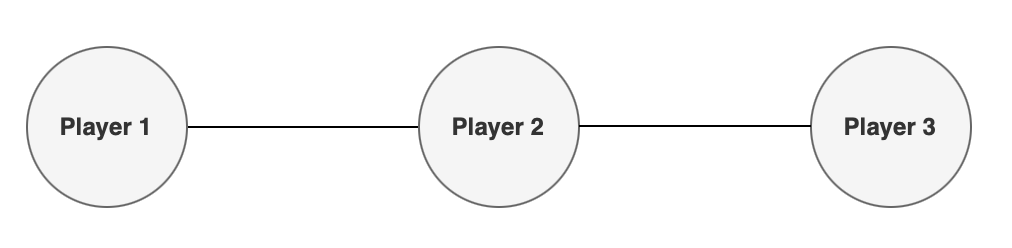
\includegraphics[width = 0.6\textwidth]{Figures/ThreePlayerNetwork.png}
    \caption{\label{fig::ThreePlayerNetwork} A NA game where the network is defined by a chain of
    three players, as described in Section \ref{sec::NonConv}.}
  \end{figure}

  As an adaptation, we take the example of a three player chain, as depicted in Figure \ref{fig::ThreePlayerNetwork}. In this example, we first assume that the network is simple (i.e. there are no self-loops and $w^{\mu \mu} = 0$). The aggregation matrix can be given as

  \begin{equation}
    W = \begin{bmatrix}
      0 & 1 & 0 \\
      w & 0 & 1 - w \\
      0 & 1 & 0
    \end{bmatrix}, \; w \in (0, 1).
  \end{equation}


  We first consider the zero-sum case to show that it does indeed converge to an equilibrium as expected. Note that the zero-sum condition given for the three player chain is given as

  \begin{equation}
    x \cdot A y + y \cdot B (w x + (1-w)z) + z \cdot C y = 0. \hspace{0.5cm} \forall x, y, z \in \Delta_1 \times \Delta_2 \times \Delta_3
  \end{equation}

  in which we use the notation that $x, y, z$ (resp. $A, B, C$) denote the strategies (resp. payoffs) of agents 1, 2 and 3 respectively. This condition is satisfied if we fix $B$ and choose

  \begin{align} \label{eq::zeroSumShapley}
    A & = - w B^T \nonumber \\
    C & = - (1 - w) B^T. 
  \end{align}

  As such in the following example, we will set $B = B_\beta$ with the choice $\beta \approx 0.576$ and set $A$ and $C$ according to the above with the choice $w \approx 0.288$. The orbits that these payoff matrices generate can be seen in Figure \ref{fig::convergentShapley}, in which, for each player, they converge to the Nash Equilibrium which, for each player, lies in the centre of the simplex.

  Let us now make the slight modification in the definition of C so that

  \begin{equation} \label{eq::nonzeroSumShapley}
    C  = - (1 - w) B, 
  \end{equation}

  with no alteration to $A$. The modification itself is small, however it results in the zero-sum
  assumption being violated. With the same choices of $\beta$ and $w$, this results in the periodic
  orbit seen in Figures \ref{fig::nonconvergentShapley}. Here,
  the orbits reach a stable limit cycle which to be centred around the interior NE.

  \begin{figure}[t]
    \centering
    \begin{subfigure}[b]{0.45 \textwidth}
      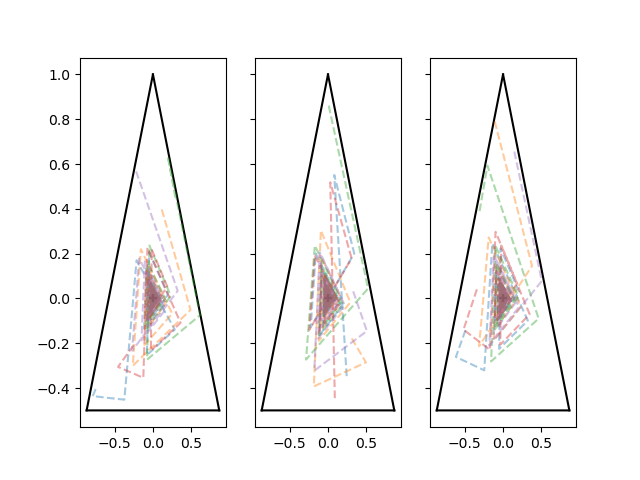
\includegraphics[width = \textwidth]{Figures/convergentShapley.png}
    \caption{\label{fig::convergentShapley}}
    \end{subfigure}
    \begin{subfigure}[b]{0.45 \textwidth}
      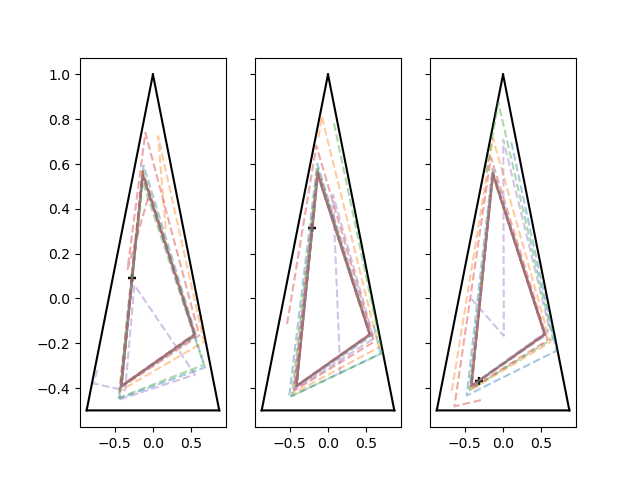
\includegraphics[width = \textwidth]{Figures/nonConvergentShapley.png}
      \caption{\label{fig::nonconvergentShapley}}
    \end{subfigure}
    \caption{\label{fig::Shapley} Orbits of the Fictitious Play in the Three Player Chain (c.f.
    Figure \ref{fig::ThreePlayerNetwork}) with payoff matrices given by (a)
    (\ref{eq::zeroSumShapley}) showing convergence to the interior NE (b)
    (\ref{eq::nonzeroSumShapley}) showing cycles around the interior NE.}
  \end{figure}

  As such, we can see that convergent behaviour is not necessarily the norm in the NA-CTFP dynamics. In fact, for the family of games discussed above, we were unable to find non-periodic behaviour for any choice of $\beta$ strictly between 0.5 and 1 for any $w$ between 0.2 and 0.8 (so that the influence of player 1 and player 3 on player 2 is not negligible). This suggests that, far from being rare, in fact NA-CTFP lends itself to an incredibly rich variety of dynamics which can be explored as future work.
  

  \subsection{Addition of Noise}

  \begin{figure}[t]
    \centering
    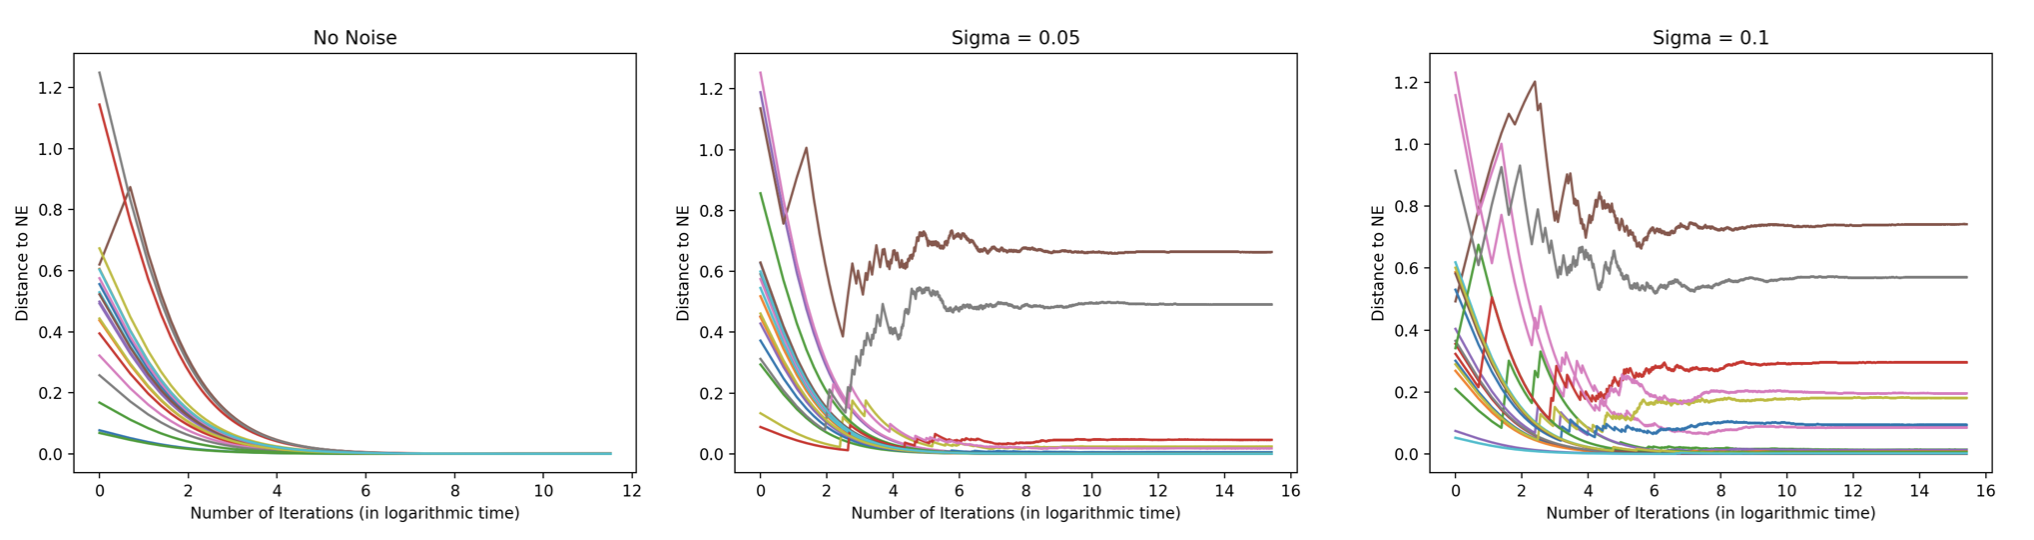
\includegraphics[width = \columnwidth]{Figures/Noise20Player.png}
    \caption{\label{fig::Noise20Player} Trajectories of NA-CTFP in a 20 player game with additive noise (Left) No noise is introduced and learning converges directly to an NE. (Middle) $\gamma = 0.05$, the trajectories converge to a fixed point but removed from the NE. (Right) $\gamma = 0.1$, the trajectories converge to a fixed point which is even further away from the NE.}
  \end{figure}

  \begin{figure}[t]
    \centering
    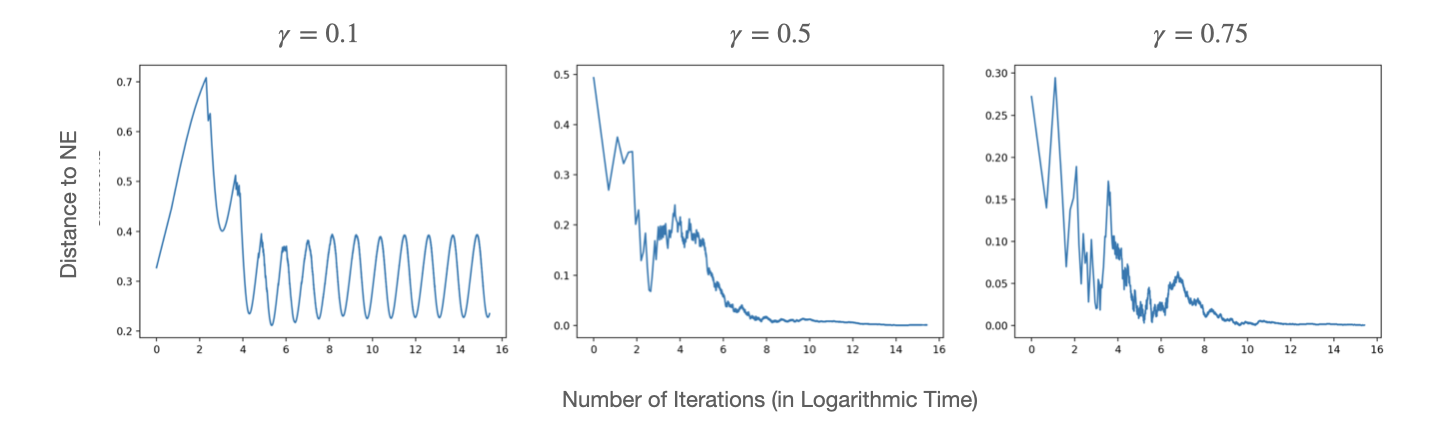
\includegraphics[width = \columnwidth]{Figures/3PlayerChainNoise.png}
    \caption{\label{fig::3PlayerChainNoise} Trajectories of NA-CTFP on the Three Player Chain of Section \ref{sec::NonConv} with additive noise. (Left) $\gamma = 0.1$ leads to a decrease in the size of the cyclic orbit (Middle) $\gamma = 0.5$, no periodicity is seen but the trajectory converges to the NE (Right) $\gamma = 0.75$, NA-CTFP still converges, though after a greater amount of time has elapsed.}
  \end{figure}

  The fictitious play process in NA games requires that, at each time step, an agent takes a
  `measurement' of the aggregate strategy of its neighbours. It is on this measurement that they
  update their own strategy. It stands to reason then, that in real environments this measurement
  may be corrupted by noise. 
  
  As such, we investigate the effect that introducing additive noise has
  on NA-CTFP in a zero-sum NA game. We do this in the following manner: at each time step, the
  reference signal $\refmu(t)$ is adjusted to $\refmu + \gamma \xi$ where $\xi$ is drawn from the
  standard normal distribution (zero mean and unit variance). By varying $\gamma$, we vary the
  strength of the noise. We vary $\gamma$ up to $0.5$ since, above this value, noisy measurements
  are likely to lie outside of the simplex. Since $\refmu$ is constrained to lie within $\Delta$, we
  can consider the range $\gamma \in [0, 0.5]$ to be the \emph{physical region}, in which noise is meaningful.

  In Figure \ref{fig::Noise20Player}, we consider a zero-sum NA game with 20 players. When there is
  no noise, it can be seen that FP reaches a fixed point which, since we set $w^{\mu \mu} = 0$,
  corresponds to an NE. After increasing $\gamma$, however, we find that the agents no longer
  converge to this NE, but rather shift away from it. What is interesting, however, is that the
  orbits do still reach a stationary state in the long run which suggests that FP is still able to
  converge with the introduction of noise.

  In Figure \ref{fig::3PlayerChainNoise} we revisit the Three Player Chain of Section
  \ref{sec::NonConv}, now under the influence of additive noise. For the sake of brevity, we only
  display the distance to the Nash Equilibrium of the first player's action, since the other agents
  behave in the same way. It can be seen that a small amount of noise has the effect of decreasing
  the size of the periodic orbit. However, as $\gamma$
  is increased to $0.5$, the algorithm seems to exhibit convergence to the NE. The implication is
  that the addition of noise may cause periodic behaviour to break and lead to the Nash Equilibrium.
  An interesting point to note is that this behaviour is in stark contrast to the replicator
  dynamic (RD) \cite{Maynard-Smith}, another adaptive algorithm linked to multi-agent learning
  \cite{CyclesAdversarialLearning}. In \cite{Imhof} and \cite{Galla}, it was found that the
  introduction of random mutations can remove convergent behaviour and instead lead to periodicity. 
  
\section{Concluding remarks}
	In this work, we have considered the action of the Fictitious Play learning algorithm in Network Aggregative Games and investigated its long term behaviour through a continuous time analysis. We find that, under a zero-sum condition, the algorithm converges to a fixed point. However, we find experimentally that this is not always the case. In fact, we find a family of NA games, based on the Shapley family, for which FP cycles about the NE. For these cases, we also perform a regret analysis which shows that, regardless of the type of game, the FP algorithm achieves no regret. 
	
	We also investigate the influence of noise on the algorithm and find that even with the introduction of additive noise, FP converges to a fixed point, though not necessarily the NE. In fact, for our cyclic family of games, we find that the introduction of noise can actually remove the periodicity, resulting in FP converging to a fixed point.
	
	Our work opens a number of lines for future work. Most notable is the effect of noise. It would be prudent to analyse this theoretically, as was done in \cite{MFGFP}, and consider the conditions under which FP will still converge to a fixed point. Furthermore, it would be interesting to investigate the phenomenon we report experimentally in a theoretical framework. Namely, the question of why noise breaks periodicity in FP and results in convergence to an NE should be investigated and, indeed, this is a line which we are currently pursuing.
	
	In addition, we note that the \emph{Mann Iteration}, a method of approximating fixed points which is investigated in \cite{Parise2020}, shares a remarkably similar structure to the discrete variant of FP. This may present an avenue by which NA-CTFP may be analysed in the case of convex cost functions. 
	
	Finally, we note that in recent years FP in two player games has shown a remarkable variety of dynamical behaviours, including periodicity and chaos. In our work we have shown convergence to a fixed point and, through experiments, periodicity. It stands to reason, therefore, that a greater variety of dynamical behaviours exist for NA-CTFP for certain classes of games. It would be important to determine what these classes are. Short from being merely a curiosity, this would allow for the identification of games in which NA-CTFP leads to inherently unpredictable behaviour, an important question from the point of view of building Safe and Trusted AI.

\section*{Broader Impact}

The dynamics of learning is an important consideration for all practitioners. In particular, it has
been shown a number of times \cite{noneqmbehaviour} that convergence of learning cannot always be
assumed. Rather, learning generally presents much more complex dynamics \cite{gallaandfarmer}, which
only increases as the number of players increases \cite{sanders}. Our work presents practitioners
who applies Fictitious Play with a case in which rigorous stability properties may be guaranteed.
We also elucidate the behaviour of the algorithm under more general assumptions, both by
understanding its regret properties as well as through an experimental study of the impact of noise.

As regards FP  itself, the learning strategy has strong applications in robotic control
\cite{Smyrnakis, Hernandez, Sharma} as well as economic modelling \cite{vonNeumann}. As such we
Furthermore, the algorithm has links to other learning protocols including the replicator dynamic
\cite{Benaim} and reinforcement learning \cite{LeslieandCollins}. Therefore, we believe that an
understanding of FP has subsequent impacts on a number of fields.

Finally, our work has a strong impact on the study of the Network Aggregative Game, which has strong
applications in multi-agent control \cite{GrammaticoAggregativeControl}. We 
believe that our work makes a strong step towards ensuring that systems which learn and adapt on
NA games maintain stability and, therefore, can be considered safe.

\begin{ack}
Use unnumbered first level headings for the acknowledgments. All acknowledgments
go at the end of the paper before the list of references. Moreover, you are required to declare 
funding (financial activities supporting the submitted work) and competing interests (related financial activities outside the submitted work). 
More information about this disclosure can be found at: \url{https://neurips.cc/Conferences/2020/PaperInformation/FundingDisclosure}.


Do {\bf not} include this section in the anonymized submission, only in the final paper. You can use the \texttt{ack} environment provided in the style file to autmoatically hide this section in the anonymized submission.
\end{ack}

\section*{References}

References follow the acknowledgments. Use unnumbered first-level heading for
the references. Any choice of citation style is acceptable as long as you are
consistent. It is permissible to reduce the font size to \verb+small+ (9 point)
when listing the references.
{\bf Note that the Reference section does not count towards the eight pages of content that are allowed.}
\medskip

\small

[1] Alexander, J.A.\ \& Mozer, M.C.\ (1995) Template-based algorithms for
connectionist rule extraction. In G.\ Tesauro, D.S.\ Touretzky and T.K.\ Leen
(eds.), {\it Advances in Neural Information Processing Systems 7},
pp.\ 609--616. Cambridge, MA: MIT Press.

[2] Bower, J.M.\ \& Beeman, D.\ (1995) {\it The Book of GENESIS: Exploring
  Realistic Neural Models with the GEneral NEural SImulation System.}  New York:
TELOS/Springer--Verlag.

[3] Hasselmo, M.E., Schnell, E.\ \& Barkai, E.\ (1995) Dynamics of learning and
recall at excitatory recurrent synapses and cholinergic modulation in rat
hippocampal region CA3. {\it Journal of Neuroscience} {\bf 15}(7):5249-5262.

\end{document}
